\section{Results}
\label{sec:results}

\subsection{Detected induction-like heads match canonical mid-layer structure}
\label{sec:result-heads}

\begin{figure}[t]
    \centering
    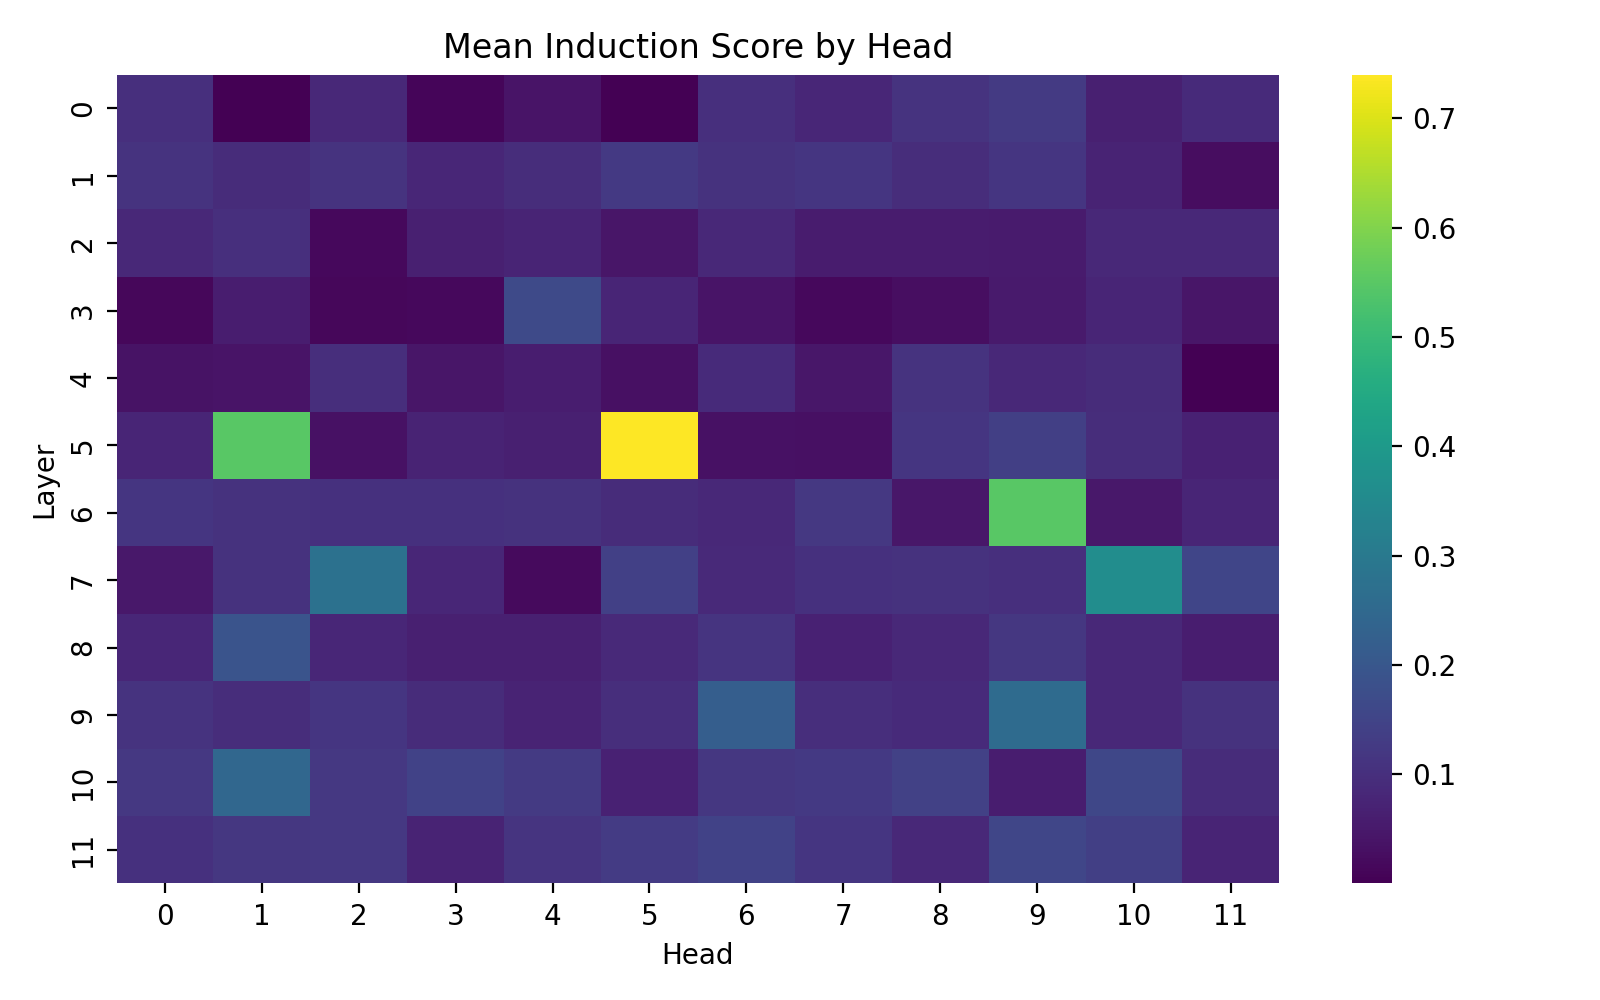
\includegraphics[width=0.78\linewidth]{figures/head_scores.png}
    \caption{Induction-head detection scores across attention heads in \gptsmall. The highest-scoring heads are concentrated in mid layers, with \headpair emerging as the top two heads in the final run. This matches the qualitative pattern reported in prior induction-head studies.}
    \label{fig:head-scores}
\end{figure}

The induction-head detector identifies a small number of clearly induction-like heads, with \headpair scoring 0.740 and 0.548 in the final run. This localization is important because it shows that the intervention targets a plausible induction circuit rather than an arbitrary collection of heads.

\subsection{Main results: bias falls, but entropy and utility fall with it}
\label{sec:main-results}

\begin{table}[t]
    \centering
    \caption{Main final-run results. Lower is better for repeated-token bias delta, KL to uniform, and WikiText perplexity. Higher is better for normalized entropy when the goal is a diffuse distribution. Best values are shown in \textbf{bold}.}
    \label{tab:main-results}
    \resizebox{\textwidth}{!}{%
    \begin{tabular}{@{}lccccc@{}}
        \toprule
        Condition & Copy accuracy & Bias delta & Normalized entropy & KL to uniform & WikiText perplexity \\
        \midrule
        Full model & 0.729 & 0.0496 & \textbf{0.860} & \textbf{0.152} & \textbf{89.9} \\
        Induction ablation (\headpair) & \textbf{0.823} & \textbf{0.0211} & 0.819 & 0.227 & 169.7 \\
        Random-head ablation (mean) & 0.723 & 0.0466 & 0.847 & 0.175 & 106.5 \\
        \bottomrule
    \end{tabular}%
    }
\end{table}


\Tabref{tab:main-results} summarizes the main final run. The strongest induction-head ablation lowers repeated-token bias delta from 0.0496 in the full model to 0.0211, a decrease of 57.5\%. Relative to the mean random-head control (0.0466), the intervention remains clearly lower. However, the same ablation also lowers normalized entropy from 0.860 to 0.819 and raises WikiText perplexity from 89.9 to 169.7. The random-head control also hurts utility, but much less severely, reaching a mean perplexity of 106.5.

The copy task adds an important complication. Ablating \headpair \emph{increases} copy-task top-1 accuracy from 0.729 to 0.823 rather than lowering it. This means the top-scoring induction-like subset in the final run is not behaving like a clean copy-only circuit. The intervention changes behavior, but not in the simple direction implied by the original hypothesis.

\begin{figure}[t]
    \centering
    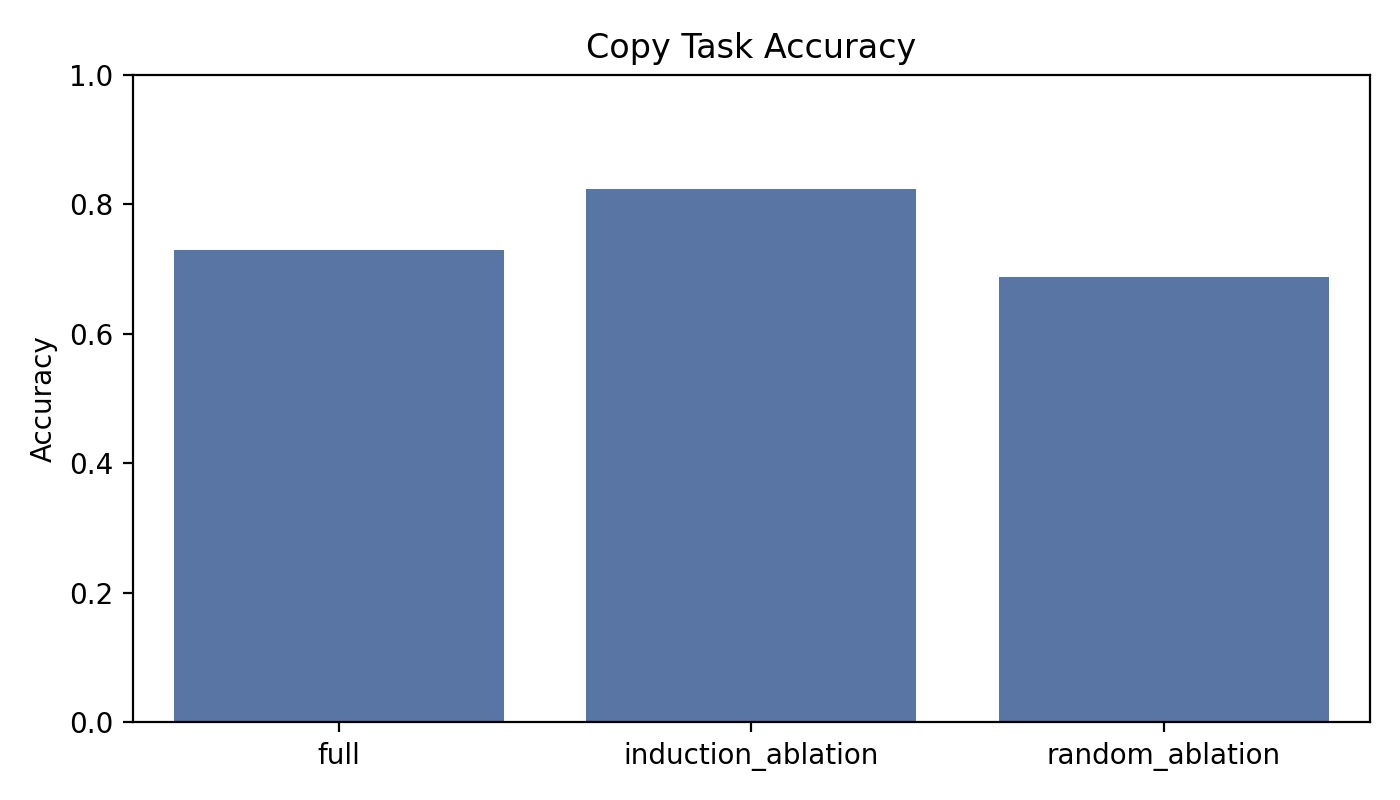
\includegraphics[width=0.72\linewidth]{figures/copy_accuracy.png}
    \caption{Copy-task accuracy across full, induction-ablation, and random-head conditions. The final run does not show a clean ``remove induction heads, reduce copying'' pattern: ablating \headpair increases copy-task accuracy above both the full model and the mean random-head control.}
    \label{fig:copy-accuracy}
\end{figure}

\begin{figure}[t]
    \centering
    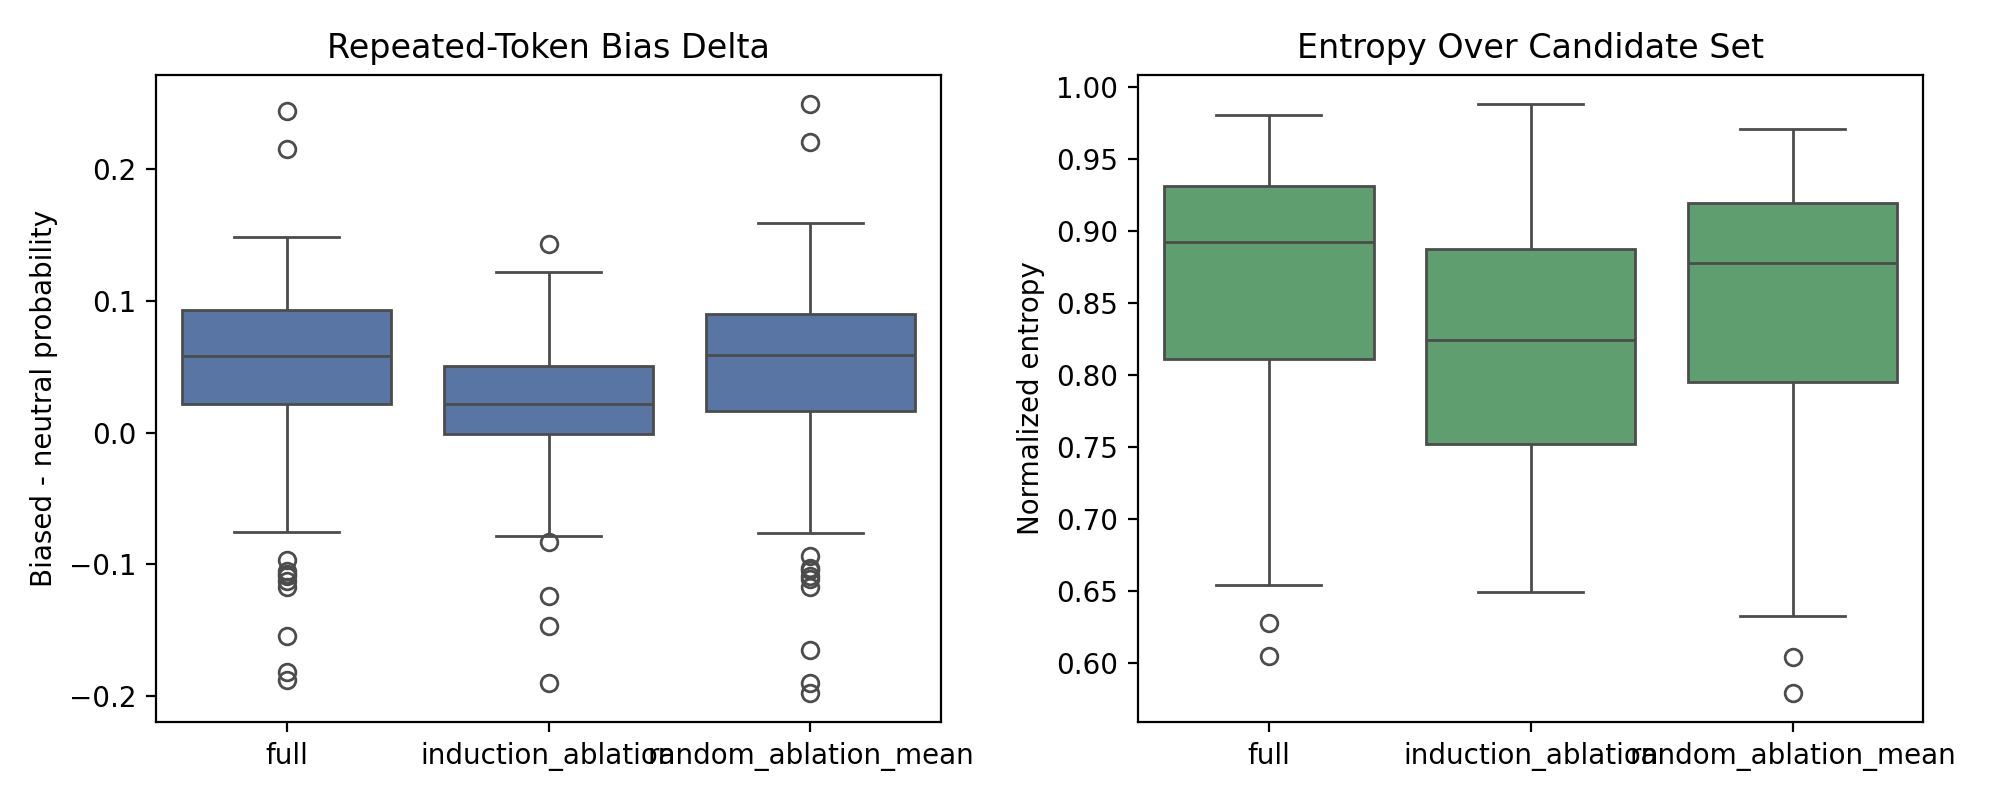
\includegraphics[width=0.92\linewidth]{figures/random_bias_entropy.png}
    \caption{Random-choice leakage metrics across conditions. Induction-head ablation lowers repeated-token bias but also lowers entropy over the valid candidate set. Lower bias therefore does not translate into more diffuse output distributions.}
    \label{fig:random-bias-entropy}
\end{figure}

\subsection{Prompt-level tests show a real effect, but not a clean mitigation}
\label{sec:stat-tests}

\begin{table}[t]
    \centering
    \caption{Prompt-level paired comparisons for the final random-choice run. Mean difference is condition A minus condition B. All tests use Wilcoxon signed-rank because the paired differences are non-normal.}
    \label{tab:stat-tests}
    \resizebox{\textwidth}{!}{%
    \begin{tabular}{@{}lcccccc@{}}
        \toprule
        Comparison & Mean diff & 95\% bootstrap CI & Test & $p$ & BH-adjusted $p$ & Effect size \\
        \midrule
        Bias delta: induction vs.\ full & \textbf{$-0.0285$} & [$-0.0400$, $-0.0172$] & Wilcoxon & $1.54\times10^{-7}$ & $4.23\times10^{-7}$ & $-0.51$ \\
        Bias delta: induction vs.\ random & \textbf{$-0.0255$} & [$-0.0370$, $-0.0145$] & Wilcoxon & $8.08\times10^{-7}$ & $1.08\times10^{-6}$ & $-0.46$ \\
        Entropy: induction vs.\ full & $-0.0417$ & [$-0.0552$, $-0.0274$] & Wilcoxon & $2.11\times10^{-7}$ & $4.23\times10^{-7}$ & $-0.59$ \\
        Entropy: induction vs.\ random & $-0.0289$ & [$-0.0430$, $-0.0142$] & Wilcoxon & $2.21\times10^{-5}$ & $2.21\times10^{-5}$ & $-0.40$ \\
        \bottomrule
    \end{tabular}%
    }
\end{table}


\Tabref{tab:stat-tests} reports paired prompt-level comparisons for the random-choice task. All four primary comparisons are significant after Benjamini-Hochberg correction. Relative to the full model, induction-head ablation lowers repeated-token bias by 0.0285 (95\% CI [$-0.0400$, $-0.0172$], Wilcoxon $p=1.54\times10^{-7}$) but also lowers normalized entropy by 0.0417 (95\% CI [$-0.0552$, $-0.0274$], Wilcoxon $p=2.11\times10^{-7}$). The comparison against the random-head control shows the same pattern: lower bias and lower entropy.

These prompt-level results matter because they rule out the simplest null hypothesis that the final-run reduction in repeated-token bias is just noise. At the same time, they also rule out the strongest positive interpretation. The intervention does not make the model more uniformly random over the valid choices. It sharpens the distribution in a different way.

\subsection{Sensitivity runs flip the causal story}
\label{sec:sensitivity}

\begin{table}[t]
    \centering
    \caption{Sensitivity runs over different high-scoring induction-like head subsets. The sign of the repeated-token bias effect changes across subsets, which is the main evidence against a monolithic leakage-circuit interpretation.}
    \label{tab:sensitivity}
    \resizebox{\textwidth}{!}{%
    \begin{tabular}{@{}lcccccccc@{}}
        \toprule
        Run & Heads & Copy acc.\ full & Copy acc.\ ablated & Bias full & Bias ablated & Entropy full & Entropy ablated & WikiText ppl ablated \\
        \midrule
        Sweep top-2 & \texttt{L5H5,L6H9} & 0.542 & 0.250 & 0.0371 & 0.0804 & 0.8701 & \textbf{0.8720} & \textbf{86.83} \\
        Sweep top-3 & \texttt{L5H5,L6H9,L5H1} & 0.542 & 0.333 & 0.0371 & 0.0638 & 0.8701 & 0.7909 & 201.45 \\
        Final run & \texttt{L5H5,L5H1} & \textbf{0.729} & \textbf{0.823} & 0.0496 & \textbf{0.0211} & 0.8602 & 0.8186 & 169.74 \\
        \bottomrule
    \end{tabular}%
    }
\end{table}


\Tabref{tab:sensitivity} is the most important result in the paper. In the smaller top-2 sensitivity run, ablating \texttt{L5H5,L6H9} drops copy accuracy from 0.542 to 0.250 but \emph{increases} repeated-token bias from 0.0371 to 0.0804. Adding \texttt{L5H1} in the top-3 run still leaves bias above the full model at 0.0638 and drives perplexity to 201.45. The final run with \headpair instead lowers bias to 0.0211 while also increasing copy accuracy.

This sign flip means that ``induction-like heads'' are not interchangeable for the purpose of leakage mitigation. Different high-scoring subsets push the model in different directions. A head can look induction-like under the detector while still playing a heterogeneous role once we intervene on actual behavior.

\begin{figure}[t]
    \centering
    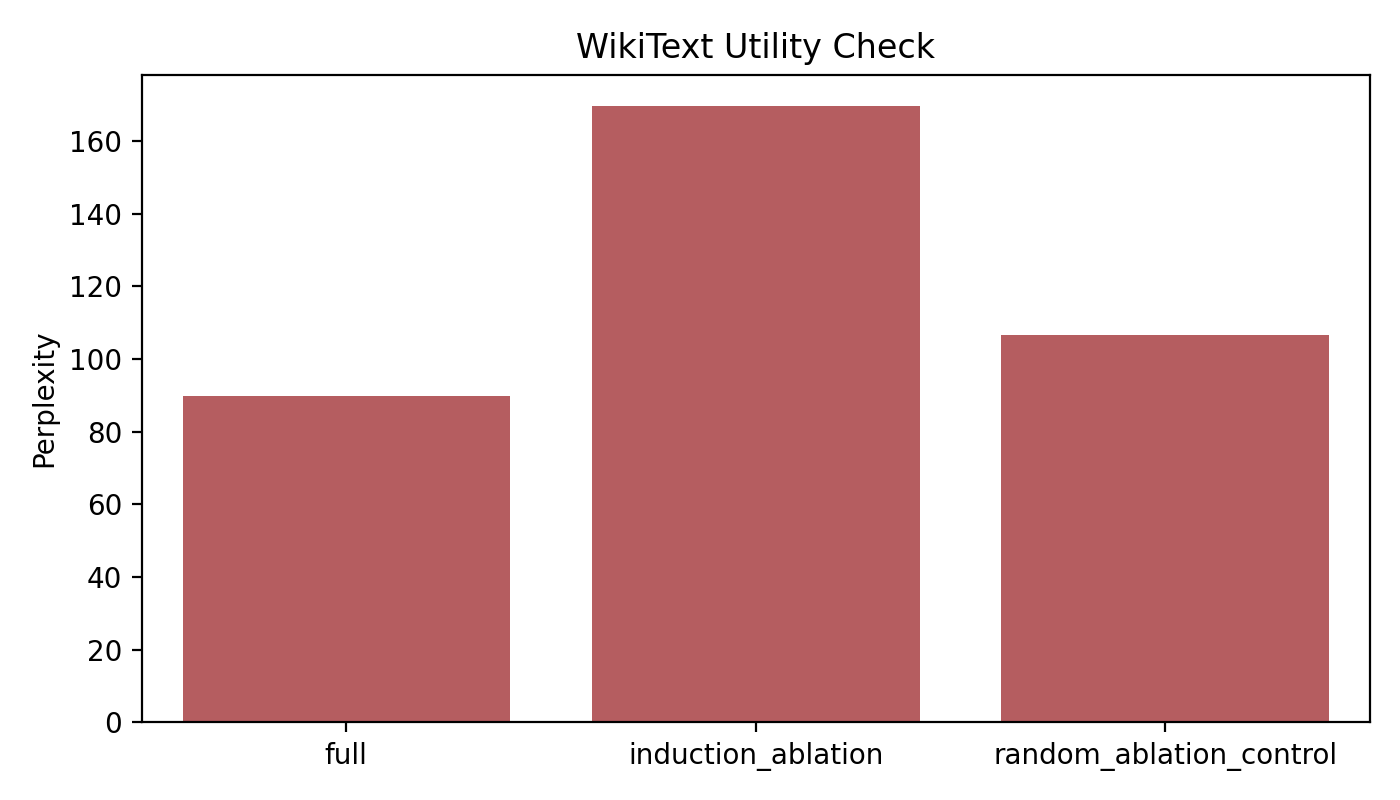
\includegraphics[width=0.72\linewidth]{figures/wikitext_perplexity.png}
    \caption{WikiText perplexity under the main intervention and random-head control. Hard ablation of the detected induction-like heads substantially harms language modeling utility, which makes the intervention unattractive as a leakage-specific fix.}
    \label{fig:wikitext-ppl}
\end{figure}
